\section{FUNDAMENTAÇÃO TEÓRICA}

\subsection{Monitoramento Aéreo Brasileiro}

Próximo aos aeroportos, os aviões são monitorados visualmente pelos controladores de voo e por radares auxiliares. Após cerca de 10 quilômetros, a aeronave passa a ser monitorada por radares de controle de aproximação (APP), que garantem uma distância mínima entre as aeronaves e previnem possíveis colisões. Fora do alcance do APP, a aeronave passa a ser monitorada pelo Departamento de Controle do Espaço Aéreo (DECEA), até chegar ao seu destino. \cite{decea}.

O DECEA tem por objetivo gerenciar as atividades no espaço aéreo brasileiro. Sua estrutura conta com quatro Centros Integrados de Defesa Aérea e Controle de Tráfego Aéreo (CINDACTA). A unidade CINDACTA I é responsável pelo espaço aéreo do Distrito Federal, Goiás, parte do Mato Grosso e Região Sudeste; a unidade CINDACTA II é responsável pela Região Sul, Mato Grosso do Sul e parte sul e oeste de São Paulo; a unidade CINDACTA III é responsável pela Região Nordeste, parte de Minas Gerais, parte do Tocantins e área oceânica que separa o Brasil da África e da Europa; e a unidade CINDACTA IV se responsabiliza pela Região Amazônica. O DECEA também conta com três subdepartamentos de supervisão, um Serviço Regional de Proteção ao Voo (SRPV), cinco Centros de Controle de Área (ACC), 47 Controles de Aproximação (APP), 59 Torres de Controle de Aeródromo (TWR), 79 Destacamentos de Controle do Espaço Aéreo (DTCEA), além das mais de 90 Estações de Telecomunicações Aeronáuticas e diversas divisões de apoio por todo o País \cite{decea}.

\subsection{Radares}

Quando estão fora do alcance dos controladores de voo, as aeronaves são monitoradas por radares. Estes aparelhos são divididos em dois tipos: os primários e os secundários. Os radares primários emitem ondas eletromagnéticas à atmosfera que retornam ao refletirem em algum obstáculo. Através da medição do tempo de ida e volta das ondas, pode-se medir a distância e posição do objeto. No entanto, radares primários não capturam dados de altitude e elevação. Os radares secundários funcionam enviando mensagens às aeronaves, que respondem com informações da posição, velocidade, altitude, etc. Para isso, é necessário que a aeronave tenha um transreceptor (aparelho capaz de receber e enviar mensagens). Caso o avião não possua esse aparelho, o radar secundário será incapaz de encontrá-lo. Muitas aeronaves em funcionamento não possuem um transreceptor abordo e, portanto, não são identificadas por radares secundários. Assim, a maioria dos aeroportos são equipados com os dois tipos de radar \cite{tecmundo}.

Radares ainda são largamente utilizados, mas são aparelhos caros e, apesar de cumprirem bem o seu trabalho, barreiras físicas e condições atmosféricas desfavoráveis podem atrapalhar seu funcionamento. A atualização do posicionamento do avião ocorre apenas a cada 30 segundos, o que dificulta a eficiência na prevenção contra acidentes e leva à necessidade de se dispor de um método de monitoramento aéreo mais confiável e acessível. Para resolver tais problemas do sistema atual de monitoramento aéreo, foi criado o sistema CNS/ATM (Comunicação, Navegação, Vigilância e Gerenciamento de Tráfego Aéreo), que usa a tecnologia ADS-B para o compartilhamento de informações das aeronaves.

\subsection{Tecnologia ADS-B}

O sistema CNS/ATM pretende dar fim aos complexos e caros sistemas baseados em radares, substituindo-os pela a tecnologia de Vigilância Segura Automática por Radiodifusão (ADS-B).

A tecnologia ADS-B baseia-se em sistemas modernos de geolocalização para detecção do posicionamento das aeronaves. Após serem coletados, os dados da aeronave são codificados em mensagens de 112 bits em formato hexadecimal e enviados em um intervalo configurável entre 0,5 e 2 segundos em todas as direções. As mensagens podem ser coletadas e propagadas por outras aeronaves, receptores posicionados no solo ou torres de controle, desde que possuam um receptor ADS-B. Mesmo que uma aeronave esteja distante de qualquer torre de controle, suas mensagens serão propagadas por outras aeronaves até chegar em algum receptor. Dessa forma, esse formato de compartilhamento aumenta consideravelmente o alcance e a precisão do monitoramento.

Apesar de ser mais barata e simples, a tecnologia ADS-B é totalmente dependente do bom funcionamento dos sistemas de geolocalização, o que os tornam elementos críticos do sistema.

\begin{figure}[H] %use h para forçar que a figura fique abaixo do texto

\caption{\label{fig:exemplo-1} Funcionamento do compartilhamento de mensagens ADS-B}

    \fbox{
        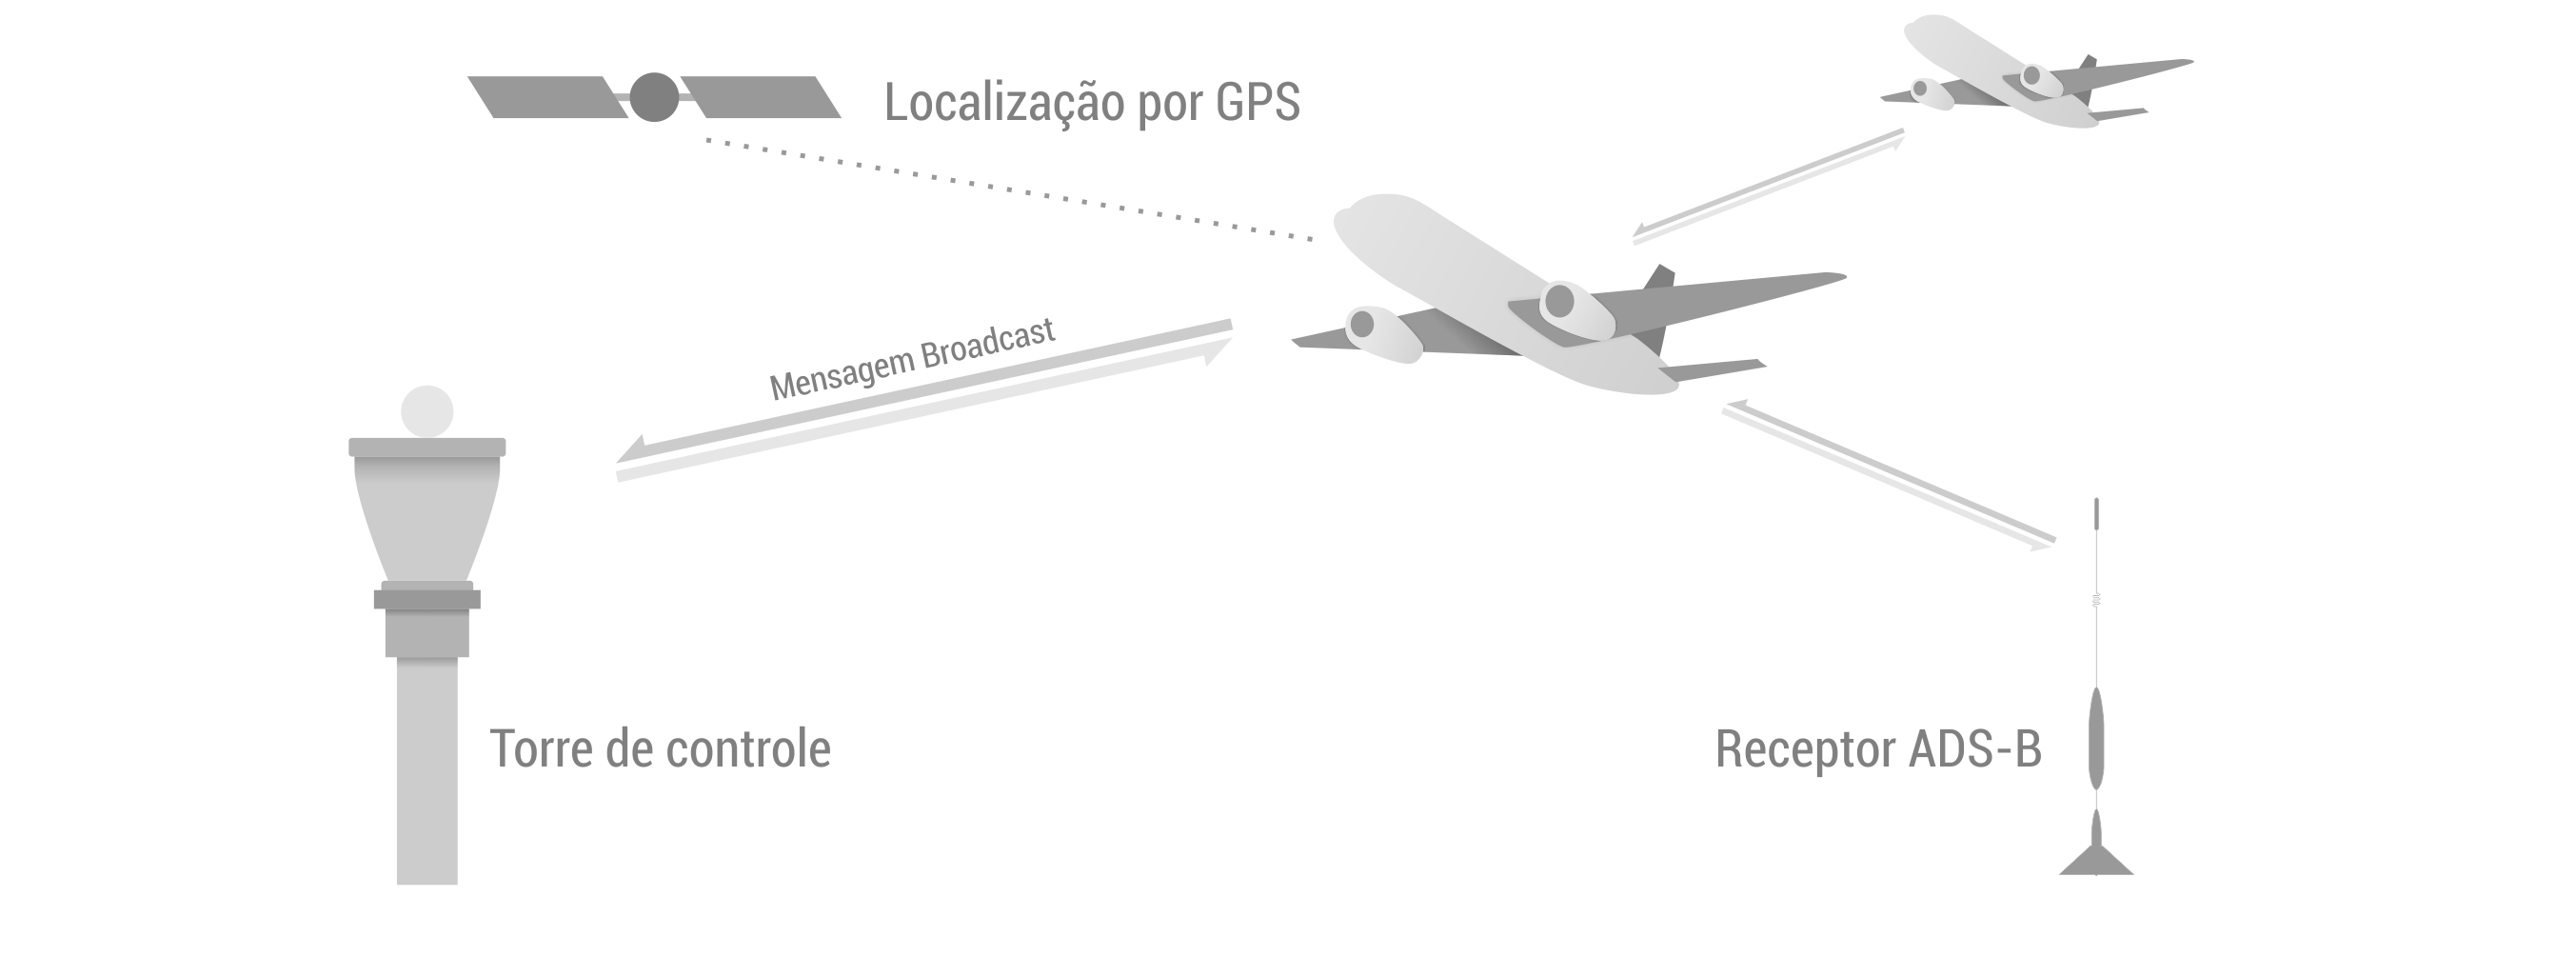
\includegraphics[scale=0.67]{figuras/ads-b} % altere o atributo scale para o tamanho da figura
    }
    
\legend{Fonte: Elaborada pelo autor}
    	
\end{figure}

\subsection{Análise e Detecção de Colisão Entre Aeronaves no Espaço Aéreo}
Com o auxílio de tecnologias modernas de coleta de dados como a ADS-B, é possível monitorar com precisão e rapidez as milhares de aeronaves que sobrevoam o planeta simultaneamente. Mas utilizar tais dados para a análise e detecção de colisão exige algoritmos em sua maioria complexos e com vários problemas de otimização. Um exemplo de algoritmo relativamente simples e eficiente é apresentado no trabalho de \citeonline{Gariel2011}, o qual será utilizado neste trabalho em testes de escalabilidade.

O algoritmo de \citeonline{Gariel2011} considera duas zonas em torno da aeronave que garantem sua segurança. A primeira zona se chama Collision Airspace Zone (CAZ), uma região cilíndrica com 160 metros de raio e 60 metros de altura, cujas dimensões consideram o tamanho das aeronaves atuais e possíveis imprecisões em sua localização. Se outra aeronave cruzar essa zona, estará correndo um risco sério de colisão. A Protection Airspace Zone (PAZ) determina uma região cilíndrica em torno da aeronave, normalmente maior que a região CAZ, que não tem seu foco em prever uma colisão iminente, mas sim proporcionar um voo confortável para o piloto, mantendo-o suficientemente distante de outros voos. Seu tamanho é calculado em função de sua velocidade relativa a uma segunda aeronave. Por tanto, a região PAZ é dinâmica e varia dependendo do par de aeronaves que está sendo verificado. As dimensões da região PAZ podem ser obtidas com:
\[ R_{PAZ}(t) = R_{PAZ, min} + max(0, V_{R}(t))\tau _{hor} \]
\[ H_{PAZ}(t) = H_{PAZ, min} + max(0, V_{R, vert}(t))\tau _{vert} \]
onde \(R_{PAZ, min} = R_{CAZ} = 160\, metros\), \(V_{R}(t)\) é a velocidade horizontal relativa entre as aeronaves no instante \(t\), \(\tau_{hor} = 10s\) é uma constante de tempo para a dimensão horizontal de PAZ, \(H_{PAZ, min} = 91\, metros\) é a altura mínima de PAZ, \(V_{R, vert}(t)\) é a velocidade vertical relativa entre as aeronaves e \(\tau_{ver} = 10s\) é uma constante de tempo para a dimensão vertical de PAZ.

O algoritmo também prevê alertas distintos para cada tipo de conflito. Caso uma aeronave esteja prestes a entrar na região PAZ de outra dentro dos próximos 15 segundos, um alerta é criado, advertindo que os aviões apresentam uma distância crítica entre si. Se o conflito for detectado para os próximos 15 segundos, outra detecção PAZ é esperada antes que o alerta seja criado, evitando que alertas sejam criados quando uma aeronave cruza momentaneamente a rota de outra. Caso o conflito seja previsto para menos de 15 segundos, o alerta e criado imediatamente. O alerta CAZ funciona de forma semelhante, mas tem muito mais gravidade por indicar uma colisão iminente.

Além de verificar posição atual do avião, o algoritmo faz uma simulação da rota que será percorrida pelo mesmo nos próximos 15 segundos, baseando-se em sua posição, velocidade e taxa de giro. O valor de \(t\) varia, por tanto, de \(0\) à \(15\), e são verificados conflitos PAZ e CAZ para cada novo valor de posição gerado em função de \(t\). Na verificação de colisão entre duas aeronaves, suas respectivas rotas serão sincronizadas em relação a \(t\) e propagadas simultaneamente. Assim, caso a primeira aeronave tenha enviado sua última informação de posição no instante \(t = 1446520500\) (\textit{timestamp} do dia 3 de novembro de 2015, às 3 horas) e a segunda tenha enviado duas informações em \(t = 1446520400\) e \(t = 1446520600\), será efetuado um cálculo de interpolação cúbica para a descoberta da posição da segunda aeronave exatamente no instante \(t = 1446520500\). A partir dessa sincronização dos valores de \(t\), será feita a simulação das rotas das duas aeronaves.

\subsection{Análise e Detecção de Colisão em Grande Escala}

Mesmo com tecnologias mais precisas para o monitoramento de aeronaves, garantir um voo seguro ainda é um grande desafio. Em seu módulo de detecção de colisão, o sistema Radar Livre pretende evitar colisões entre aeronaves e entre aeronaves e acidentes geográficos, utilizando as informações coletadas por seus receptores ADS-B. No entanto, se o sistema for alimentado com um grande número de aeronaves, o módulo de detecção de colisão irá lidar com um grande problema de escalabilidade. Segundo o site Flightradar24\footnote{www.flightradar24.com}, onde podemos acompanhar o voo de aeronaves em tempo real, às 9h30min do dia 24 de Maio de 2016 eram registradas pouco mais de 12.500 aeronaves em funcionamento ao redor do mundo. Ressalta-se que as aeronaves identificadas eram apenas aquelas que carregavam um transreceptor ADS-B e estavam no raio de alcance de alguma antena do sistema. Portanto essa quantidade deve estar bem abaixo do número real de aeronaves em pleno voo no momento da verificação. Verificar a possibilidade de colisão em tantas aeronaves de forma rápida e eficiente é o principal desafio do módulo de detecção de colisão do sistema Radar Livre.

O sistema TCAS funciona dentro da aeronave e preocupa-se em evitar colisão apenas com as aeronaves vizinhas, não necessitando de uma grande capacidade de processamento na verificação de poucas aeronaves. O sistema Radar Livre utiliza uma base de dados unificada com informações de todas as aeronaves observadas, o que obriga seu módulo de detecção de colisão a analisar a possibilidade de colisão entre todas as aeronaves registradas pelo sistema. Em um espaço aéreo pequeno cruzado por três aviões A, B e C, por exemplo, para detectar com segurança todas as possíveis colisões seria necessário analisar um possível conflito entre os aviões A e B, entre B e C e entre A e C, totalizando 3 verificações. Em uma espaço aéreo com 12.500 aeronaves, seriam necessárias 78.118.750 verificações. Se considerarmos que para se ter um monitoramento preciso devemos atualizar todas as previsões a cada 2 segundos, e que em média 12.500 aeronaves sobrevoam simultaneamente a qualquer hora, chegaremos a 337.730.000.000 verificações diárias e o problema de escalabilidade fica claro.

